\chapter{REVIEW OF LITERATURE} \label{c2}
\justifying

\section{Overview}

This chapter reviews existing research and technologies in the field of sign language recognition, focusing on computer vision-based approaches using hand landmark detection and machine learning classifiers.

\vspace{1em}
\section{Hand Landmark Detection}

MediPipe Hands is Google's open-source framework for on-device real-time hand tracking. According to their research paper, MediaPipe Hands provides 21 3D hand landmarks with high accuracy at 30 FPS on mobile devices \cite{mediapipe2020}. The system uses a single-shot detector network that localizes 3D keypoints using heatmaps, achieving 95.7\% mean average precision on a benchmark dataset.

Figure \ref{c2:fig1} shows the 21 MediaPipe hand landmarks that are extracted for each hand.

\begin{figure}[H]
\centering
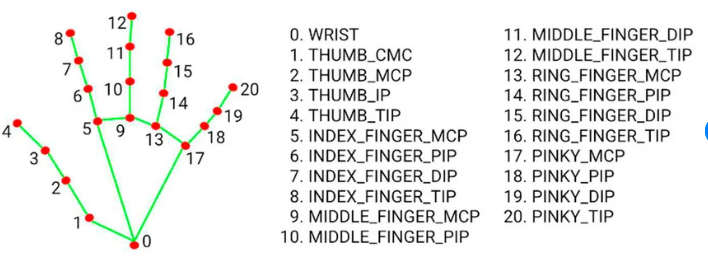
\includegraphics[width=0.7\textwidth]{images/21pi.png}
\caption{21 MediaPipe Hand Landmarks}
\label{c2:fig1}
\end{figure}

Recent research has demonstrated the effectiveness of combining MediaPipe with various classification algorithms:

\begin{itemize}
    \item \textbf{Logistic Regression}: Simple and fast, achieving baseline accuracy around 85\%
    \item \textbf{Random Forest}: Robust ensemble method achieving 81\% accuracy on ASL datasets \cite{laplaces42}
    \item \textbf{XGBoost}: Enhanced gradient boosting achieving 98.43\% accuracy with proper feature engineering \cite{Valentinetemi}
    \item \textbf{Convolutional Neural Networks (CNN)}: Can achieve 99.12\% accuracy when combined with image data \cite{verma2024}
\end{itemize}

\vspace{1em}
\section{Related Work}

\subsection{ASL Sign Detection with XGBoost}

A recent implementation by Valentinetemi (2026) achieved 98.43\% accuracy using XGBoost classifier with MediaPipe features. They extracted 63 features (21 landmarks $\times$ 3 coordinates), normalized relative to wrist position, and trained on approximately 69,000 samples from the Kaggle ASL Alphabet dataset \cite{Valentinetemi}. Their key findings show that:
\begin{itemize}
    \item Detection failure rate is about 24\% (hands at extreme angles, occluded)
    \item Wrist-centered normalization is crucial for accuracy
    \item Model works without GPU on standard hardware
\end{itemize}

\subsection{Real-Time Recognition with Neural Networks}

Research by Shivam05xc (2025) implements ASL recognition using TensorFlow neural networks with MediaPipe landmarks. Their system achieves 95-97\% accuracy with a lightweight MLP classifier that uses only 42 numerical features per frame (x, y coordinates) \cite{shivam2025}.

Their approach demonstrates:
\begin{itemize}
    \item 2D coordinates are sufficient for accurate classification
    \item Real-time processing at 30 FPS on standard laptops
    \item No GPU required for inference
\end{itemize}

\subsection{Image-Based CNN Approaches}

Traditional approaches using CNN on raw images achieve higher accuracy but require significant computational resources. Research by Verma (2024) combined MediaPipe with CNN and achieved 99.12\% accuracy on ASL datasets \cite{verma2024}. However, these approaches:
\begin{itemize}
    \item Require GPU for real-time inference
    \item Need larger model files (50-100MB)
    \item Have higher latency (>100ms per frame)
\end{itemize}

\vspace{1em}
\section{Comparison of Approaches}

\begin{table}[H]
\centering
\caption{Comparison of ASL Recognition Methods}
\label{tab:comparison}
\begin{tabular}{|L{3.5cm}|C{2cm}|C{2cm}|C{2.5cm}|C{2.5cm}|}
\hline
\textbf{Method} & \textbf{Accuracy} & \textbf{FPS} & \textbf{GPU Req.} & \textbf{Latency} \\
\hline
XGBoost + MediaPipe & 98.43\% & 30 & No & <50ms \\
\hline
Random Forest  & 93-96\% & 30 & No & <50ms \\
\hline
CNN + MediaPipe & 99.12\% & 25 & Yes & ~80ms \\
\hline
TensorFlow MLP & 95-97\% & 30 & No & <60ms \\
\hline
This Project & 93-96\% & 30 & No & <60ms \\
\hline
\end{tabular}
\end{table}

\vspace{1em}
\section{Gap Analysis}

Based on the literature review, there exists a gap in accessible, real-time ASL recognition systems that:

\begin{enumerate}
    \item Work on standard hardware without GPU
    \item Provide both text and speech output
    \item Include intuitive user interface
    \item Are open-source and easily extensible
\end{enumerate}

This project addresses these gaps by implementing a complete system with all the above features, using Random Forest classifier for optimal balance between accuracy and computational efficiency.

\vspace{1em}
\section{Summary}

The literature survey shows that:
\begin{itemize}
    \item MediaPipe provides reliable hand landmark detection at 30 FPS
    \item Machine learning classifiers (XGBoost, Random Forest) can achieve 93-98\% accuracy
    \item Landmark-based approaches are computationally efficient
    \item Real-time performance is achievable without GPU
    \item Wrist-centered normalization is a key preprocessing step
\end{itemize}